% Created by tikzDevice version 0.12.3.1 on 2021-05-09 13:07:50
% !TEX encoding = UTF-8 Unicode
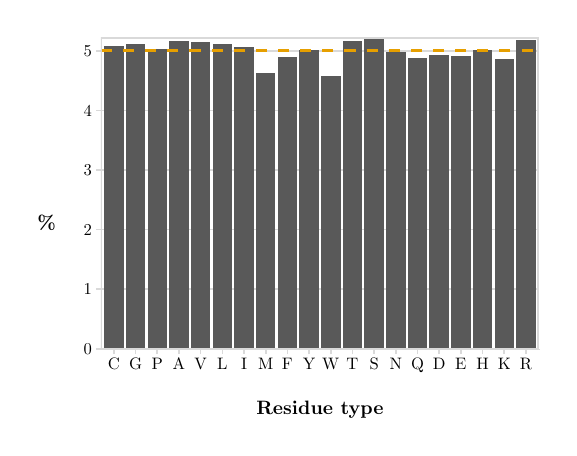
\begin{tikzpicture}[x=1pt,y=1pt]
\definecolor{fillColor}{RGB}{255,255,255}
\path[use as bounding box,fill=fillColor,fill opacity=0.00] (0,0) rectangle (188.25,144.54);
\begin{scope}
\path[clip] ( 26.46, 28.30) rectangle (184.75,141.04);
\definecolor{drawColor}{gray}{0.85}

\path[draw=drawColor,line width= 0.6pt,line join=round] ( 26.46, 28.53) --
	(184.75, 28.53);

\path[draw=drawColor,line width= 0.6pt,line join=round] ( 26.46, 50.06) --
	(184.75, 50.06);

\path[draw=drawColor,line width= 0.6pt,line join=round] ( 26.46, 71.59) --
	(184.75, 71.59);

\path[draw=drawColor,line width= 0.6pt,line join=round] ( 26.46, 93.12) --
	(184.75, 93.12);

\path[draw=drawColor,line width= 0.6pt,line join=round] ( 26.46,114.65) --
	(184.75,114.65);

\path[draw=drawColor,line width= 0.6pt,line join=round] ( 26.46,136.18) --
	(184.75,136.18);
\definecolor{fillColor}{gray}{0.35}

\path[fill=fillColor] ( 27.63, 28.53) rectangle ( 34.69,137.91);

\path[fill=fillColor] ( 35.47, 28.53) rectangle ( 42.52,138.61);

\path[fill=fillColor] ( 43.31, 28.53) rectangle ( 50.36,136.91);

\path[fill=fillColor] ( 51.14, 28.53) rectangle ( 58.20,139.61);

\path[fill=fillColor] ( 58.98, 28.53) rectangle ( 66.03,139.51);

\path[fill=fillColor] ( 66.81, 28.53) rectangle ( 73.87,138.61);

\path[fill=fillColor] ( 74.65, 28.53) rectangle ( 81.70,137.61);

\path[fill=fillColor] ( 82.49, 28.53) rectangle ( 89.54,128.31);

\path[fill=fillColor] ( 90.32, 28.53) rectangle ( 97.38,134.01);

\path[fill=fillColor] ( 98.16, 28.53) rectangle (105.21,136.41);

\path[fill=fillColor] (106.00, 28.53) rectangle (113.05,126.90);

\path[fill=fillColor] (113.83, 28.53) rectangle (120.89,139.81);

\path[fill=fillColor] (121.67, 28.53) rectangle (128.72,140.82);

\path[fill=fillColor] (129.51, 28.53) rectangle (136.56,135.71);

\path[fill=fillColor] (137.34, 28.53) rectangle (144.39,133.71);

\path[fill=fillColor] (145.18, 28.53) rectangle (152.23,134.51);

\path[fill=fillColor] (153.01, 28.53) rectangle (160.07,134.41);

\path[fill=fillColor] (160.85, 28.53) rectangle (167.90,136.61);

\path[fill=fillColor] (168.69, 28.53) rectangle (175.74,133.31);

\path[fill=fillColor] (176.52, 28.53) rectangle (183.58,140.21);
\definecolor{drawColor}{RGB}{230,159,0}

\path[draw=drawColor,line width= 1.1pt,dash pattern=on 4pt off 4pt ,line join=round] ( 26.46,136.18) -- (184.75,136.18);
\definecolor{drawColor}{gray}{0.85}

\path[draw=drawColor,line width= 1.1pt,line join=round,line cap=round] ( 26.46, 28.30) rectangle (184.75,141.04);
\end{scope}
\begin{scope}
\path[clip] (  0.00,  0.00) rectangle (188.25,144.54);
\definecolor{drawColor}{RGB}{0,0,0}

\node[text=drawColor,anchor=base east,inner sep=0pt, outer sep=0pt, scale=  0.60] at ( 23.21, 26.46) {0};

\node[text=drawColor,anchor=base east,inner sep=0pt, outer sep=0pt, scale=  0.60] at ( 23.21, 47.99) {1};

\node[text=drawColor,anchor=base east,inner sep=0pt, outer sep=0pt, scale=  0.60] at ( 23.21, 69.52) {2};

\node[text=drawColor,anchor=base east,inner sep=0pt, outer sep=0pt, scale=  0.60] at ( 23.21, 91.05) {3};

\node[text=drawColor,anchor=base east,inner sep=0pt, outer sep=0pt, scale=  0.60] at ( 23.21,112.58) {4};

\node[text=drawColor,anchor=base east,inner sep=0pt, outer sep=0pt, scale=  0.60] at ( 23.21,134.11) {5};
\end{scope}
\begin{scope}
\path[clip] (  0.00,  0.00) rectangle (188.25,144.54);
\definecolor{drawColor}{gray}{0.85}

\path[draw=drawColor,line width= 0.6pt,line join=round] ( 24.71, 28.53) --
	( 26.46, 28.53);

\path[draw=drawColor,line width= 0.6pt,line join=round] ( 24.71, 50.06) --
	( 26.46, 50.06);

\path[draw=drawColor,line width= 0.6pt,line join=round] ( 24.71, 71.59) --
	( 26.46, 71.59);

\path[draw=drawColor,line width= 0.6pt,line join=round] ( 24.71, 93.12) --
	( 26.46, 93.12);

\path[draw=drawColor,line width= 0.6pt,line join=round] ( 24.71,114.65) --
	( 26.46,114.65);

\path[draw=drawColor,line width= 0.6pt,line join=round] ( 24.71,136.18) --
	( 26.46,136.18);
\end{scope}
\begin{scope}
\path[clip] (  0.00,  0.00) rectangle (188.25,144.54);
\definecolor{drawColor}{gray}{0.85}

\path[draw=drawColor,line width= 0.6pt,line join=round,line cap=rect] ( 26.46, 28.30) --
	(184.75, 28.30);
\end{scope}
\begin{scope}
\path[clip] (  0.00,  0.00) rectangle (188.25,144.54);
\definecolor{drawColor}{gray}{0.85}

\path[draw=drawColor,line width= 0.6pt,line join=round] ( 31.16, 26.55) --
	( 31.16, 28.30);

\path[draw=drawColor,line width= 0.6pt,line join=round] ( 39.00, 26.55) --
	( 39.00, 28.30);

\path[draw=drawColor,line width= 0.6pt,line join=round] ( 46.83, 26.55) --
	( 46.83, 28.30);

\path[draw=drawColor,line width= 0.6pt,line join=round] ( 54.67, 26.55) --
	( 54.67, 28.30);

\path[draw=drawColor,line width= 0.6pt,line join=round] ( 62.50, 26.55) --
	( 62.50, 28.30);

\path[draw=drawColor,line width= 0.6pt,line join=round] ( 70.34, 26.55) --
	( 70.34, 28.30);

\path[draw=drawColor,line width= 0.6pt,line join=round] ( 78.18, 26.55) --
	( 78.18, 28.30);

\path[draw=drawColor,line width= 0.6pt,line join=round] ( 86.01, 26.55) --
	( 86.01, 28.30);

\path[draw=drawColor,line width= 0.6pt,line join=round] ( 93.85, 26.55) --
	( 93.85, 28.30);

\path[draw=drawColor,line width= 0.6pt,line join=round] (101.69, 26.55) --
	(101.69, 28.30);

\path[draw=drawColor,line width= 0.6pt,line join=round] (109.52, 26.55) --
	(109.52, 28.30);

\path[draw=drawColor,line width= 0.6pt,line join=round] (117.36, 26.55) --
	(117.36, 28.30);

\path[draw=drawColor,line width= 0.6pt,line join=round] (125.20, 26.55) --
	(125.20, 28.30);

\path[draw=drawColor,line width= 0.6pt,line join=round] (133.03, 26.55) --
	(133.03, 28.30);

\path[draw=drawColor,line width= 0.6pt,line join=round] (140.87, 26.55) --
	(140.87, 28.30);

\path[draw=drawColor,line width= 0.6pt,line join=round] (148.70, 26.55) --
	(148.70, 28.30);

\path[draw=drawColor,line width= 0.6pt,line join=round] (156.54, 26.55) --
	(156.54, 28.30);

\path[draw=drawColor,line width= 0.6pt,line join=round] (164.38, 26.55) --
	(164.38, 28.30);

\path[draw=drawColor,line width= 0.6pt,line join=round] (172.21, 26.55) --
	(172.21, 28.30);

\path[draw=drawColor,line width= 0.6pt,line join=round] (180.05, 26.55) --
	(180.05, 28.30);
\end{scope}
\begin{scope}
\path[clip] (  0.00,  0.00) rectangle (188.25,144.54);
\definecolor{drawColor}{RGB}{0,0,0}

\node[text=drawColor,anchor=base,inner sep=0pt, outer sep=0pt, scale=  0.60] at ( 31.16, 20.92) {C};

\node[text=drawColor,anchor=base,inner sep=0pt, outer sep=0pt, scale=  0.60] at ( 39.00, 20.92) {G};

\node[text=drawColor,anchor=base,inner sep=0pt, outer sep=0pt, scale=  0.60] at ( 46.83, 20.92) {P};

\node[text=drawColor,anchor=base,inner sep=0pt, outer sep=0pt, scale=  0.60] at ( 54.67, 20.92) {A};

\node[text=drawColor,anchor=base,inner sep=0pt, outer sep=0pt, scale=  0.60] at ( 62.50, 20.92) {V};

\node[text=drawColor,anchor=base,inner sep=0pt, outer sep=0pt, scale=  0.60] at ( 70.34, 20.92) {L};

\node[text=drawColor,anchor=base,inner sep=0pt, outer sep=0pt, scale=  0.60] at ( 78.18, 20.92) {I};

\node[text=drawColor,anchor=base,inner sep=0pt, outer sep=0pt, scale=  0.60] at ( 86.01, 20.92) {M};

\node[text=drawColor,anchor=base,inner sep=0pt, outer sep=0pt, scale=  0.60] at ( 93.85, 20.92) {F};

\node[text=drawColor,anchor=base,inner sep=0pt, outer sep=0pt, scale=  0.60] at (101.69, 20.92) {Y};

\node[text=drawColor,anchor=base,inner sep=0pt, outer sep=0pt, scale=  0.60] at (109.52, 20.92) {W};

\node[text=drawColor,anchor=base,inner sep=0pt, outer sep=0pt, scale=  0.60] at (117.36, 20.92) {T};

\node[text=drawColor,anchor=base,inner sep=0pt, outer sep=0pt, scale=  0.60] at (125.20, 20.92) {S};

\node[text=drawColor,anchor=base,inner sep=0pt, outer sep=0pt, scale=  0.60] at (133.03, 20.92) {N};

\node[text=drawColor,anchor=base,inner sep=0pt, outer sep=0pt, scale=  0.60] at (140.87, 20.92) {Q};

\node[text=drawColor,anchor=base,inner sep=0pt, outer sep=0pt, scale=  0.60] at (148.70, 20.92) {D};

\node[text=drawColor,anchor=base,inner sep=0pt, outer sep=0pt, scale=  0.60] at (156.54, 20.92) {E};

\node[text=drawColor,anchor=base,inner sep=0pt, outer sep=0pt, scale=  0.60] at (164.38, 20.92) {H};

\node[text=drawColor,anchor=base,inner sep=0pt, outer sep=0pt, scale=  0.60] at (172.21, 20.92) {K};

\node[text=drawColor,anchor=base,inner sep=0pt, outer sep=0pt, scale=  0.60] at (180.05, 20.92) {R};
\end{scope}
\begin{scope}
\path[clip] (  0.00,  0.00) rectangle (188.25,144.54);
\definecolor{drawColor}{RGB}{0,0,0}

\node[text=drawColor,anchor=base,inner sep=0pt, outer sep=0pt, scale=  0.70] at (105.60,  4.86) {\bfseries Residue type};
\end{scope}
\begin{scope}
\path[clip] (  0.00,  0.00) rectangle (188.25,144.54);
\definecolor{drawColor}{RGB}{0,0,0}

\node[text=drawColor,anchor=base,inner sep=0pt, outer sep=0pt, scale=  0.70] at (  6.85, 71.44) {\bfseries \%};
\end{scope}
\end{tikzpicture}%
